\documentclass{article}
\PassOptionsToPackage{hyphens}{url}
\usepackage[hidelinks]{hyperref}
\usepackage{amsmath}
\usepackage{amsthm}
\usepackage{amssymb}
\usepackage{pgfplots}
\usepackage{algpseudocode}
\newcommand{\QED}{\hfill {\qed}}
\newcommand\tab[1][1cm]{\hspace*{#1}}
\usepackage{mathtools}
\DeclarePairedDelimiter\ceil{\lceil}{\rceil}
\DeclarePairedDelimiter\floor{\lfloor}{\rfloor}
\graphicspath{ {./imgs/} }

\title{\#3 Assignment - CMPT 405}
\author{Luiz Fernando Peres de Oliveira - 301288301 - lperesde@sfu.ca}

\begin{document}

\maketitle
\textbf{\#1a)}
\\
Let $G_1$ be a graph with two vertices $A$ and $B$ and an edge $(A, B)$ with weight $1$. For every shortest path tree $T_v$, $v \in V$, $T_v$ is also a MST (it is easy to see, as there is only one tree).
\\
\\

\includegraphics[scale=0.6]{simple_graph_hw3}
\\
\\
\textbf{\#1b)}
\\
Let $G_2$ be a graph with vertices $A, B, C$ and $D$ and edges $(A, B), (A, D), (A,C), (B,C)$ and $(C,D)$, with weights $8, 4, 6, 4 \text{ and } 8$, respectively. Then, no shortest path tree $T_v$ given by Dijkstra's algorithm is a MST.
\\
\\
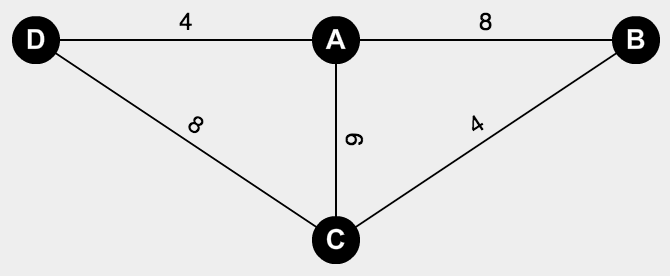
\includegraphics[scale=0.4]{complex_graph_hw3}
\\
\\
MST $= (A,C), (A,D), (B,C)$
\\
$T_a = (A, B), (A, C), (A, D)$
\\
$T_b = (A, B), (A, D), (B, C)$
\\
$T_c = (A, C), (B, C), (C, D)$
\\
$T_d = (A, B), (A, D), (C, D)$
\\
\\
\textbf{\#2)}
\\
\textbf{\#3)}
\\
\textbf{\#4)}
\\
\textbf{\#5)}
\\
\textbf{References}
\\
\end{document}